\documentclass{article}
\usepackage{setspace}
\usepackage{listings}
\usepackage{color}
\usepackage{amsmath}
\usepackage{amssymb}
\usepackage{amsthm}
\usepackage{graphicx} 
\usepackage{float} 
\usepackage{fancyhdr}                                
\usepackage{lastpage}                                           
\usepackage{layout}   
\usepackage{subfigure} 
\definecolor{codegreen}{rgb}{0,0.6,0}
\definecolor{codegray}{rgb}{0.5,0.5,0.5}
\definecolor{codepurple}{rgb}{0.58,0,0.82}
\definecolor{backcolour}{rgb}{0.95,0.95,0.92}

\lstdefinestyle{mystyle}{
    backgroundcolor=\color{backcolour},   
    commentstyle=\color{codegreen},
    keywordstyle=\color{magenta},
    numberstyle=\tiny\color{codegray},
    stringstyle=\color{codepurple},
    basicstyle=\footnotesize,
    breakatwhitespace=false,         
    breaklines=true,                 
    captionpos=b,                    
    keepspaces=true,                 
    numbers=left,                    
    numbersep=5pt,                  
    showspaces=false,                
    showstringspaces=false,
    showtabs=false,                  
    tabsize=2
}
\pagestyle{fancy}  
\lhead{ZHANG HUAKANG}
\chead{Assignment 1} 
\rhead{DB92760} 
\renewcommand{\baselinestretch}{1.05}
\title{Assignment 1 of CISC 2002}
\author{ZHANG Huakang/DB92760}

\newcommand\decbin[9]{%
\par\smallskip
\makebox[3cm][r]{$#1$\ }\fbox{#2}\,\fbox{#3}\,\fbox{#4}\,\fbox{#5}\,\fbox{#6}\,\fbox{#7}\,\fbox{#8}\,\fbox{#9}\par}


\def\unsignedbytecalc#1{%
\par\smallskip
\noindent$#1_{10}$\par
\smallskip
\gdef\result{}%
$\left.\begin{array}{r@{\quad}|c}\udbc{#1}\end{array}\right\}\result$\par}

\makeatletter

\def\udbc#1{%
\ifnum#1=\z@
\expandafter\@gobble
\else
\expandafter\@firstofone
\fi
{2)\!\underline{\,#1}&\edef\r{\ifodd#1 1\else 0\fi}\r\xdef\result{\r\result}\\
\expandafter\udbc\expandafter{\the\numexpr(\ifodd#1 #1-1\else#1\fi)/2\relax}%
}}

\begin{document}
    \maketitle
    \section{}
        \unsignedbytecalc{114}
        \begin{equation*}
            \begin{split}
                0.25\times 2= 0.5 |&0\\
                0.5\times 2 = 1|& 1\\
            \end{split}
        \end{equation*}
        $$0.25_{10}=0.01_2$$
        \begin{equation*}
            \begin{split}
                -114.25=&-1110010.01\\
                    =&-1.11001001\times 2^6\\
                    =&(-1)^{1}\times 2^6 \times 1.11001001\\
                    s=&1\\
                    e-127=&6\\
                    e=&133\\
                    f=&11001001
            \end{split}
        \end{equation*}
        \newpage
        \unsignedbytecalc{133}
        The  representation  of $-114.25$ in IEEE single precision formatis is $$1100\;0010\;1110\;0100\;0000\;0000\;0000\;0000$$
    \section{}
        $$0100 \; 0011\; 0101\; 0100\; 0000\; 0000\; 0000\; 0000$$
        \begin{equation*}
            \begin{split}
                s=&0\\
                e=&10000110_2\\
                    =&134\\
                f=&101 01\\
                (-1)^s\times2^{e-127}\times1.101 01
                    =&2^7\times1.101 01\\
                    =&11010100_2\\
                    =&212\\
            \end{split}
        \end{equation*}
    \section{}
        \subsection{}
            \begin{equation*}
                \begin{split}
                    \frac{1}{5}\times 2 =0.4 &| 0\\
                    0.4\times 2=0.8 &| 0\\
                    0.8\times 2 =1.6 &|1\\
                    0.6\times 2 = 1.2 &|1\\
                    0.2\times 2=0.4&|0\\
                    ...\\
                    ...\\
                    ...\\
                \end{split}
            \end{equation*}
            $$\frac{1}{5}_{10}=0.\dot{0}01\dot{1}_2$$
        \subsection{}
            $$-9.6=(-1)^1\times 2^3 \times 1.2$$
            \begin{equation*}
                \begin{split}
                    s=&1\\
                    e-127=&3\\
                        e&=130_{10}=10000010_2\\
                    1.f=&1.\dot{0}01\dot{1}_2
                \end{split}
            \end{equation*}
            The  representation  of $-9.6$ in IEEE single precision formatis is 
            $$1100\; 0001\; 0001\; 1001\; 1001\; 1001\; 1001\; 1001$$
        \subsection{}
            \begin{align*}
                1100 &\;0001 &\;0001&\;1001&\;1001&\;1001&\;1001&\;1001\\
                C&\;    1&\; 1&\; 9&\;  9&\; 9&\;  9&\;  9
            \end{align*}
    \section{}
        \subsection{}
            By L'Hospital's rule,
            \begin{equation*}
                \begin{split}
                    \lim_{x\rightarrow 0}f(a)=&\lim_{x\rightarrow 0}\frac{\sqrt{2+x}-\sqrt{2-x}}{2x}\\
                        =&\lim_{x\rightarrow 0}\frac{\frac{1}{2}(\frac{1}{\sqrt{2+x}}+\frac{1}{\sqrt{2-x}})}{2}\\
                        =&\frac{\frac{1}{\sqrt{2}}}{2}\\
                        =&\frac{\sqrt{2}}{4}
                \end{split}
            \end{equation*}
        \subsection{}
        \subsection{}
            \begin{proof}
                \begin{equation*}
                    \begin{split}
                        f(x)=&\frac{\sqrt{2+x}-\sqrt{2-x}}{2x}\\
                            =&\frac{(\sqrt{2+x}-\sqrt{2-x})(\sqrt{2+x}+\sqrt{2-x})}{2x(\sqrt{2+x}+\sqrt{2-x})}\\
                            =&\frac{2+x-(2-x)}{2x(\sqrt{2+x}+\sqrt{2-x})}\\
                            =&\frac{2x}{2x(\sqrt{2+x}+\sqrt{2-x})}\\
                            =&\frac{1}{\sqrt{2+x}+\sqrt{2-x}}\\
                    \end{split}
                \end{equation*}
            \end{proof}
        \subsection{}
\lstinputlisting[language=Matlab,style=mystyle,caption=Assignments1-4.4.m]{code/Assignments1.m}
\begin{figure}[H] 
    \centering 
    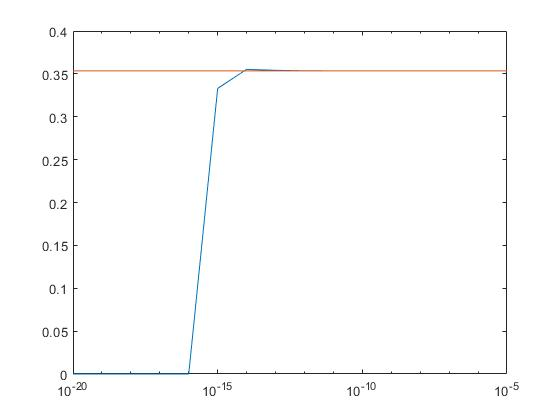
\includegraphics[width=0.7\textwidth]{img/Assignement.jpg}
    \caption{Output} 
\end{figure}
\end{document}

